\documentclass[12pt,titlepage]{article}

\setlength{\oddsidemargin}{0in}
\setlength{\evensidemargin}{0in}
\setlength{\textwidth}{6.5in}
%
\setlength{\textheight}{9in}
\setlength{\topmargin}{0in}
\setlength{\headsep}{0in}
\setlength{\topskip}{0in}
\setlength{\headheight}{0in}

\usepackage{graphicx}
\usepackage{times}
\usepackage[plainpages=false, colorlinks=true, anchorcolor=blue, linkcolor=blue, citecolor=blue, bookmarks=false, urlcolor=blue]
{hyperref}
\usepackage[square,comma,authoryear]{natbib}


\title{DOE Office of Science INCITE Project:\\
{\it Extreme-scale Simulation of Supernovae and Magnetars from Realistic Progenitors}\\
2018 Q3 Report}

\author{Principal Investigator:\\Sean M. Couch\\
  Michigan State University \vspace{0.1in}\\
  Co-Investigators: \\
  Andrew Christlieb (Michigan State University) \\
  Evan O'Connor (Stockholm University)\\
  Kuo-Chuan Pan (Michigan State University) \\
  Luke Roberts (Michigan State University) \\
  MacKenzie Warren (Michigan State University) \\
}

\date{October 1, 2018}


\begin{document}


\maketitle


%%%%%%%%%%%%%%%%%%%%%%%%%%%%%%%%%
\section{Project Usage}

%%%%%%%%%%%%%%%%%%%


\begin{figure}
  \begin{tabular}{cc}
    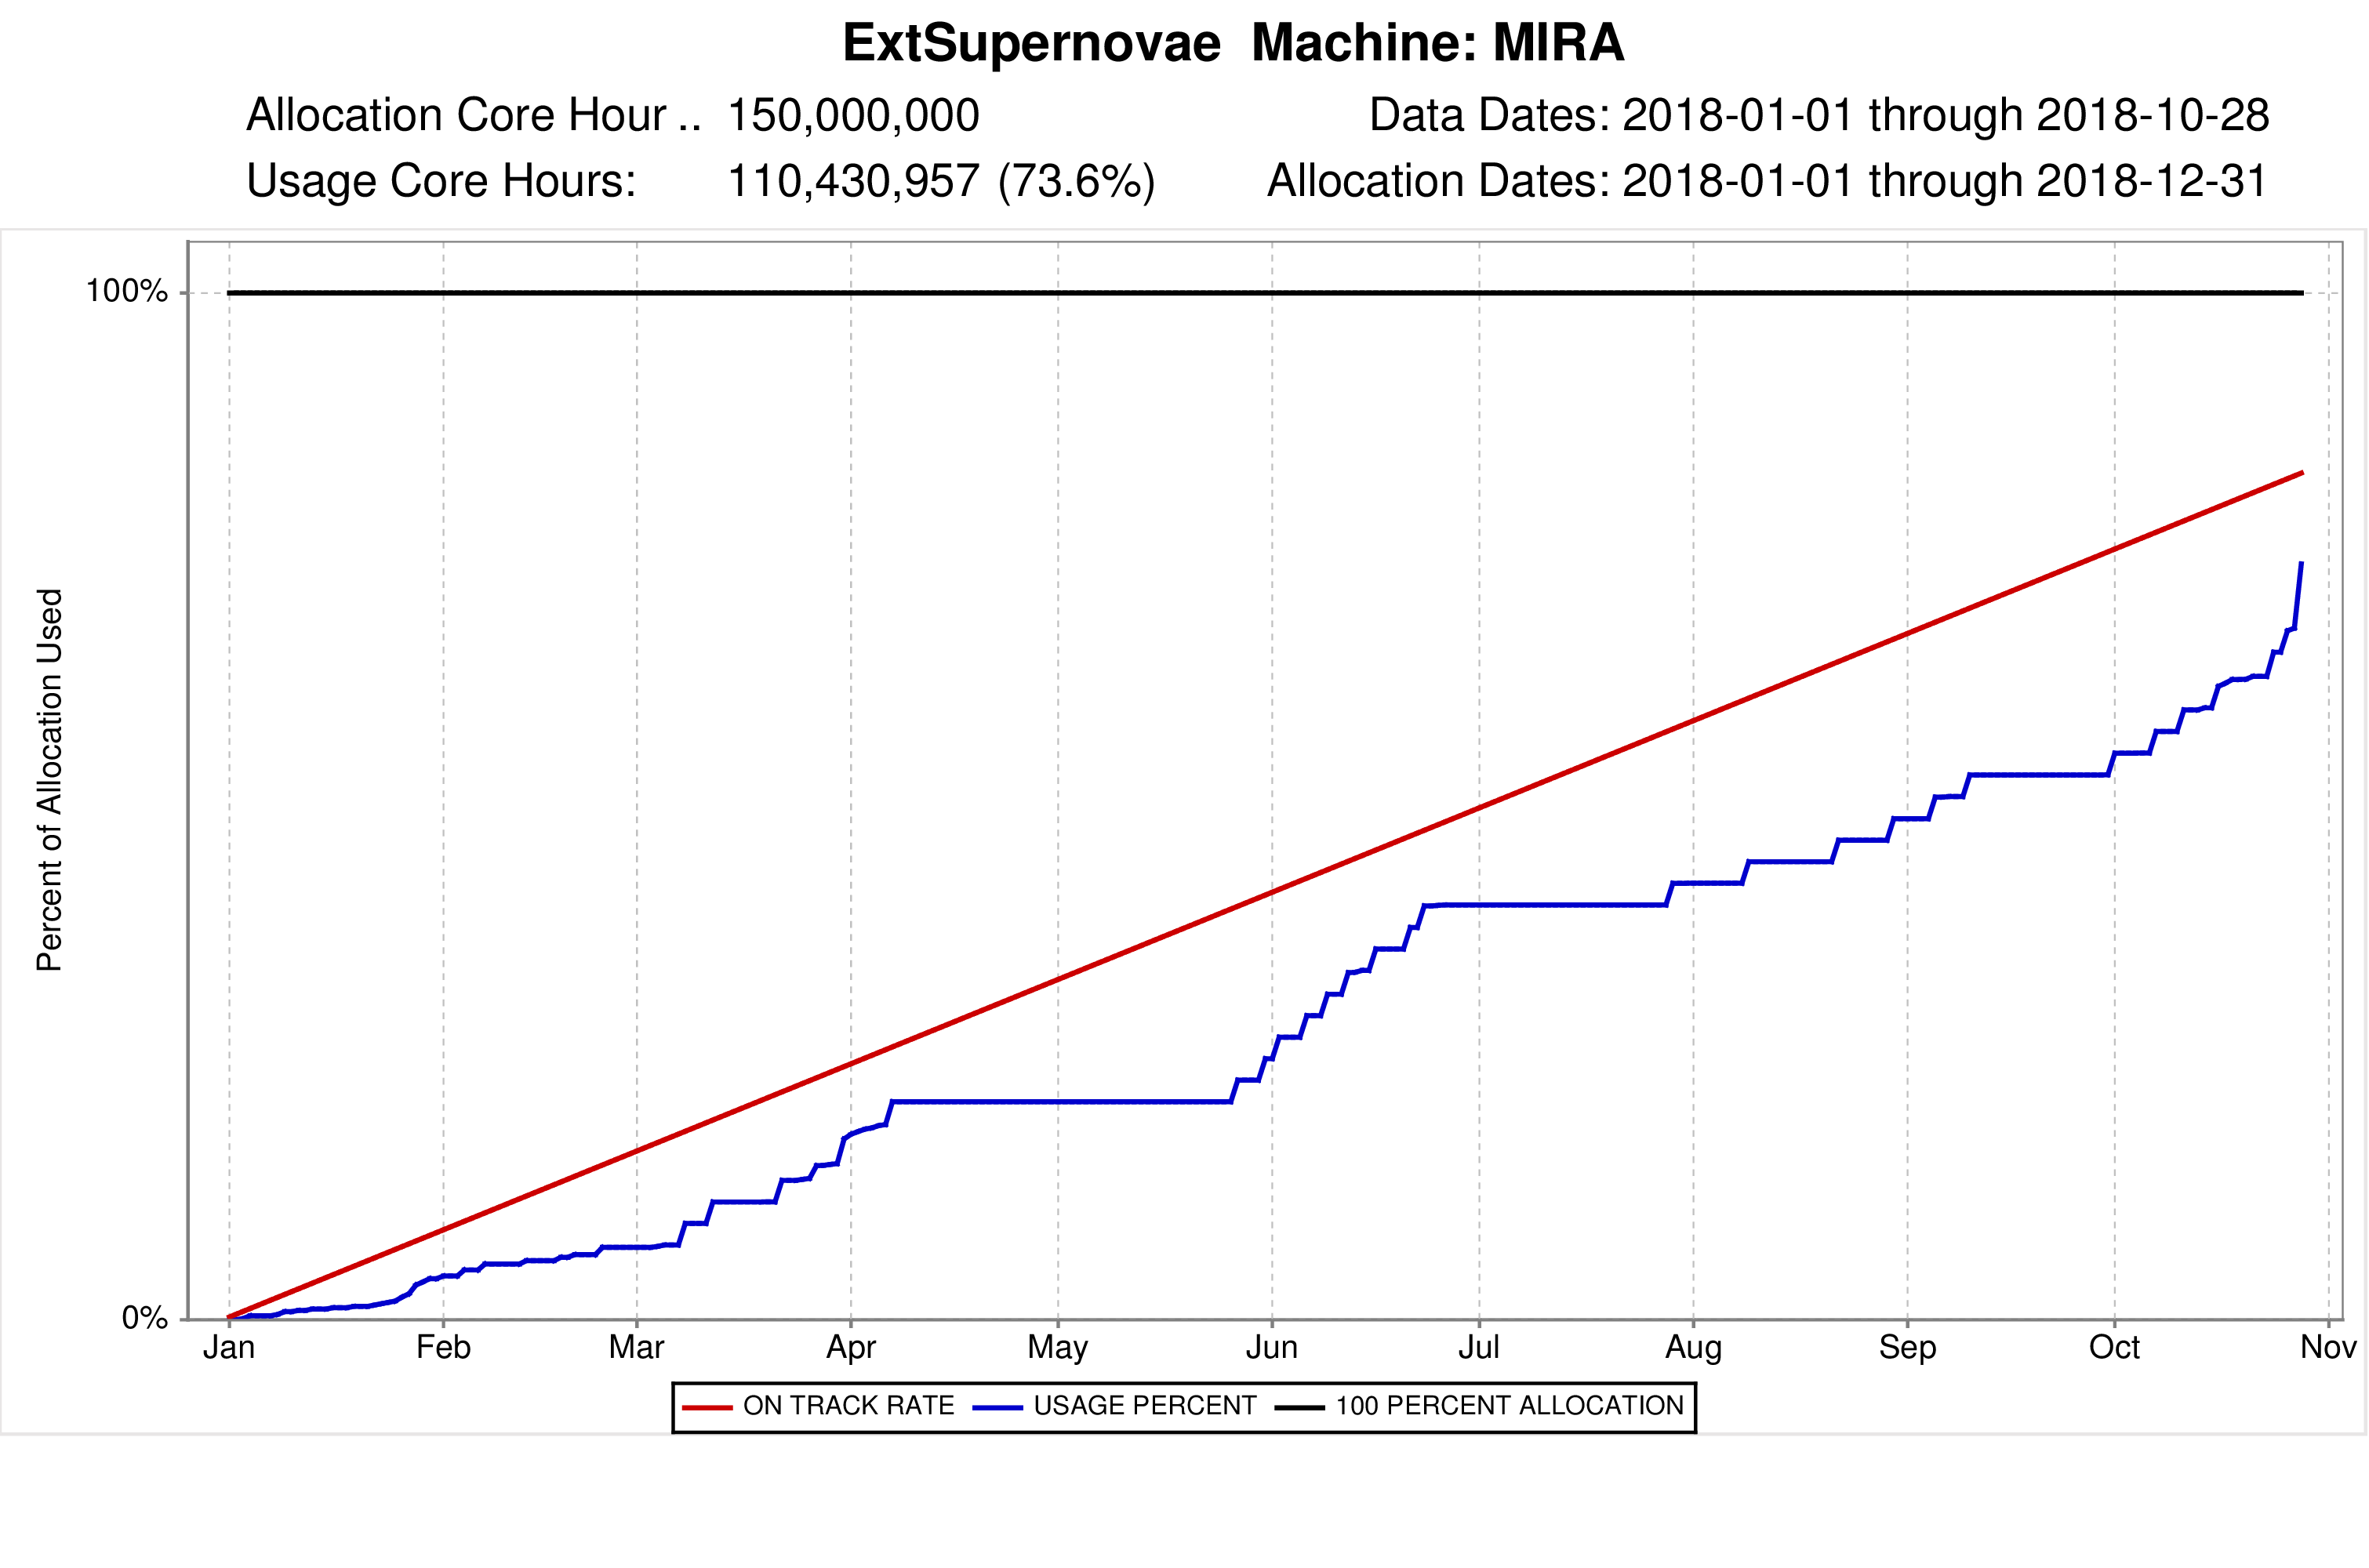
\includegraphics[width=3.25in]{on_track_graph_mira.png}
    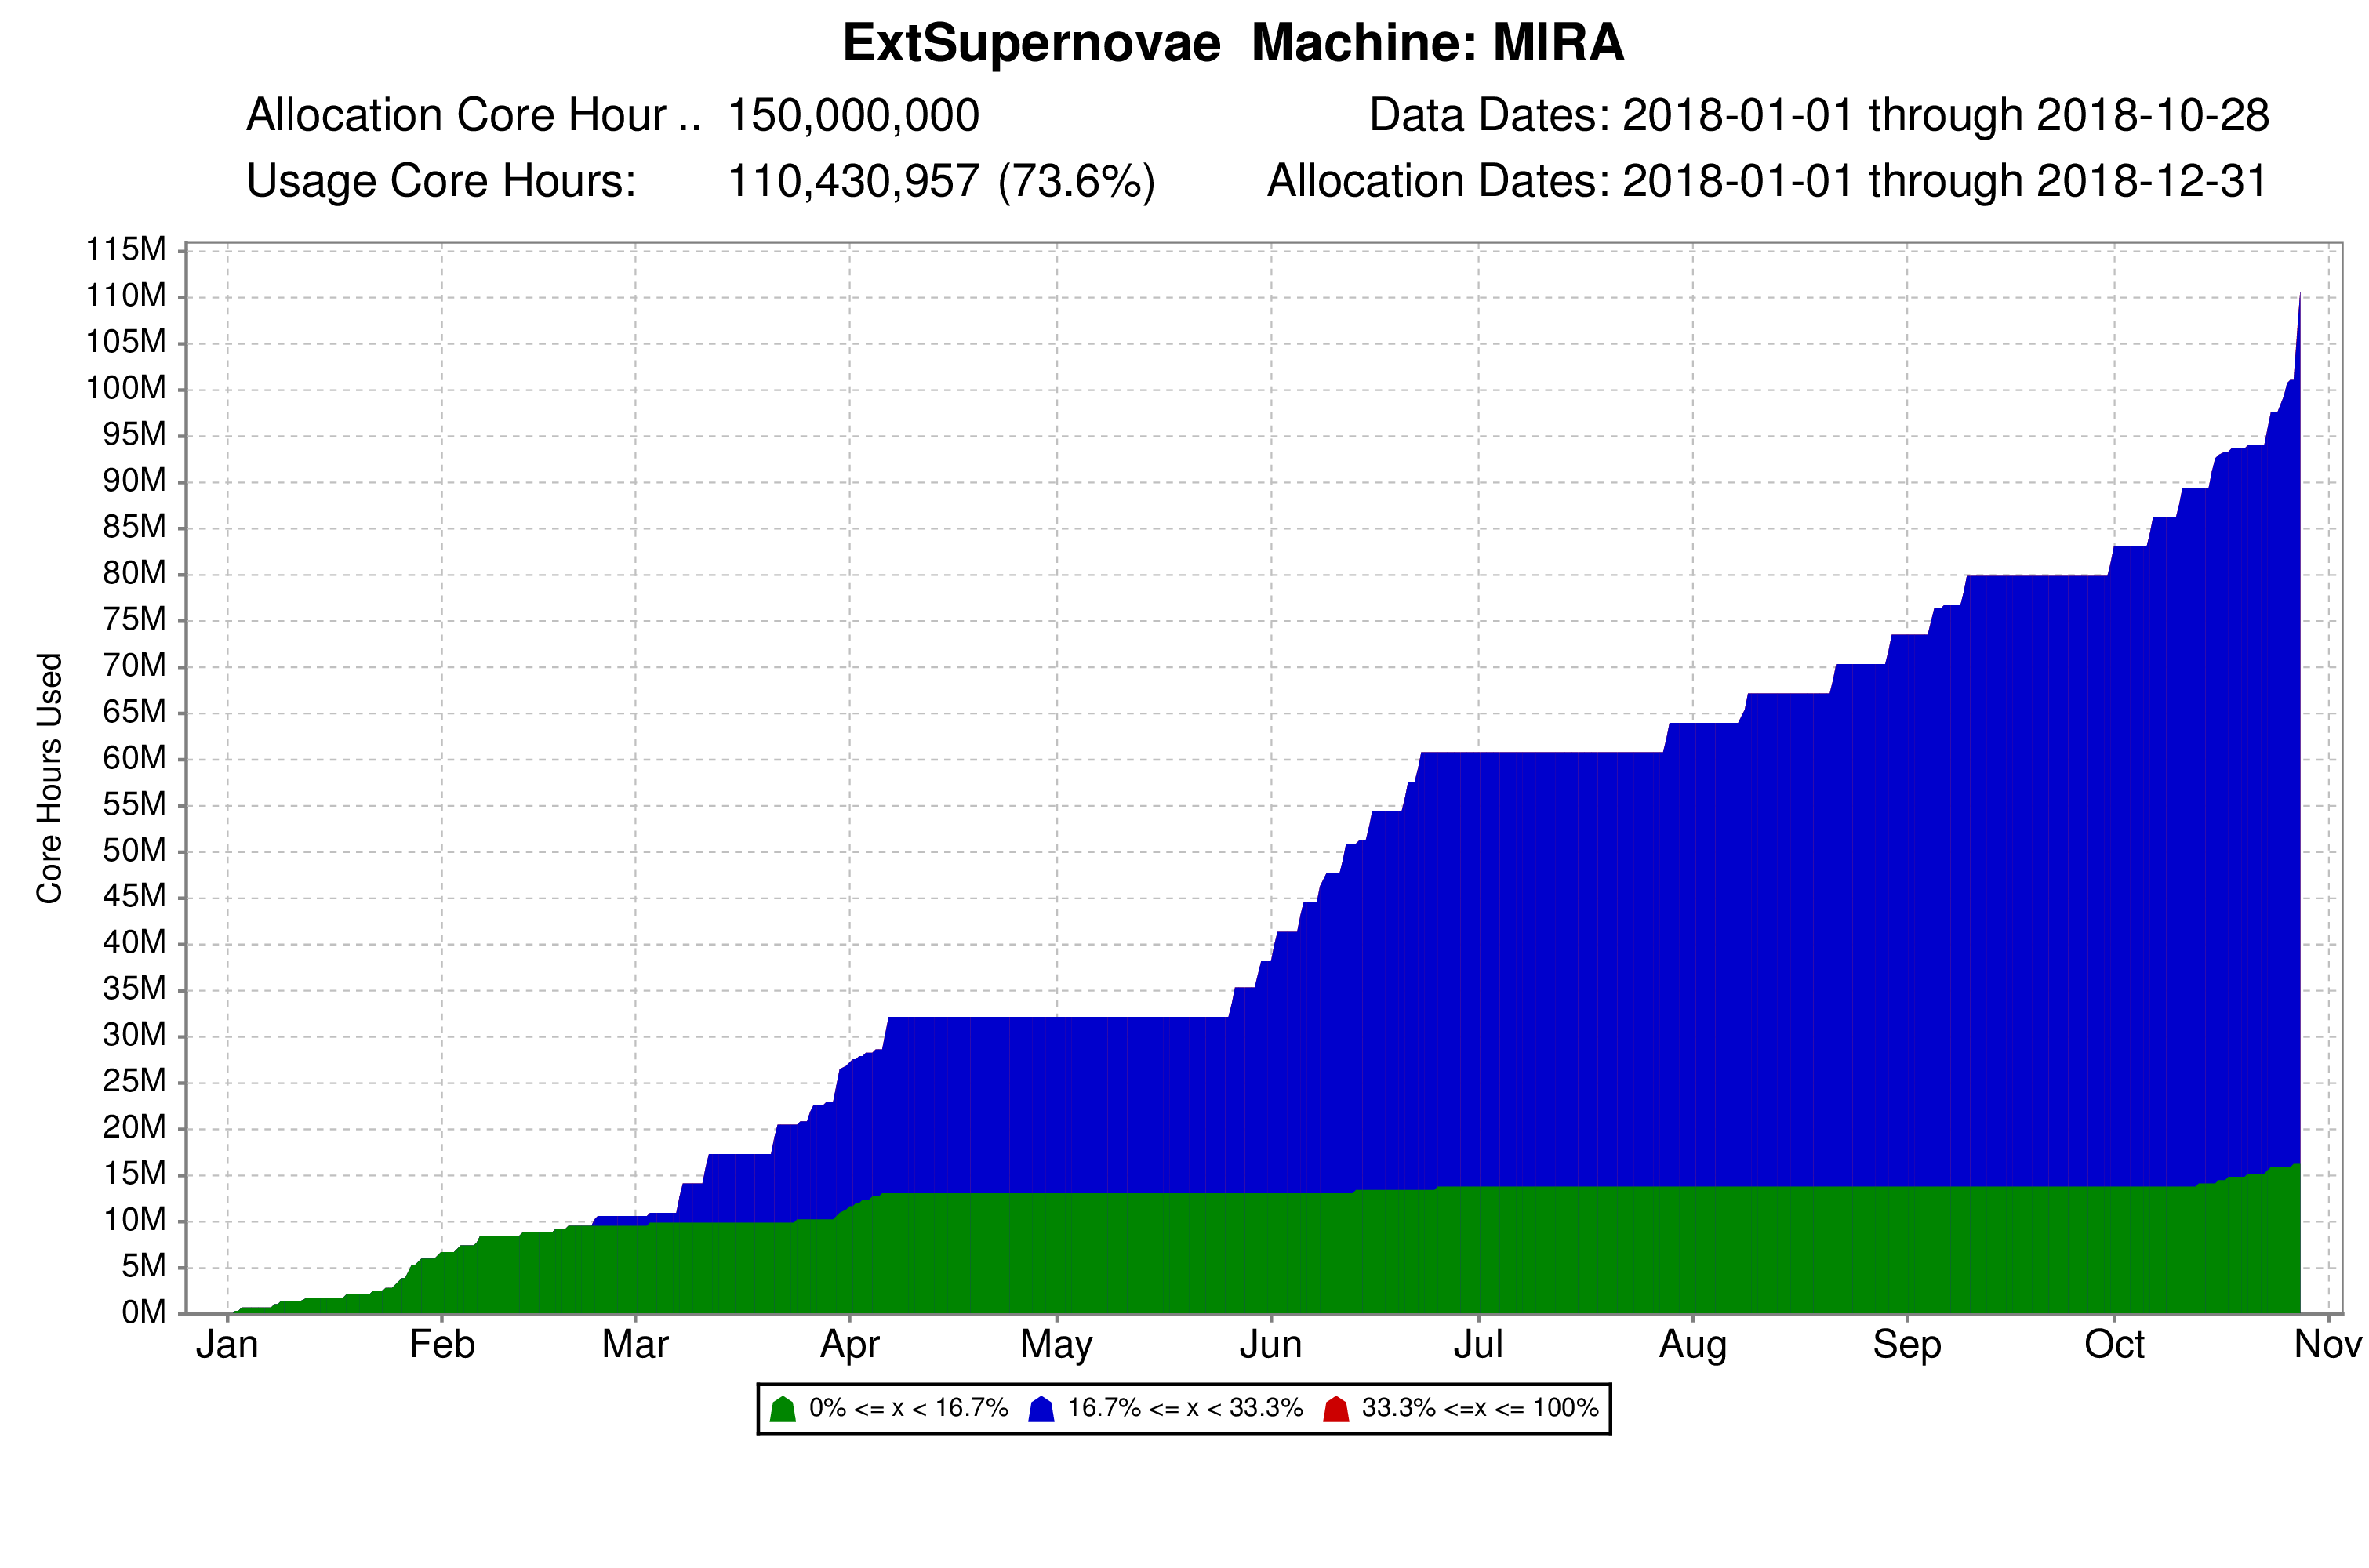
\includegraphics[width=3.25in]{categorized_hours_graph_mira.png} \\
    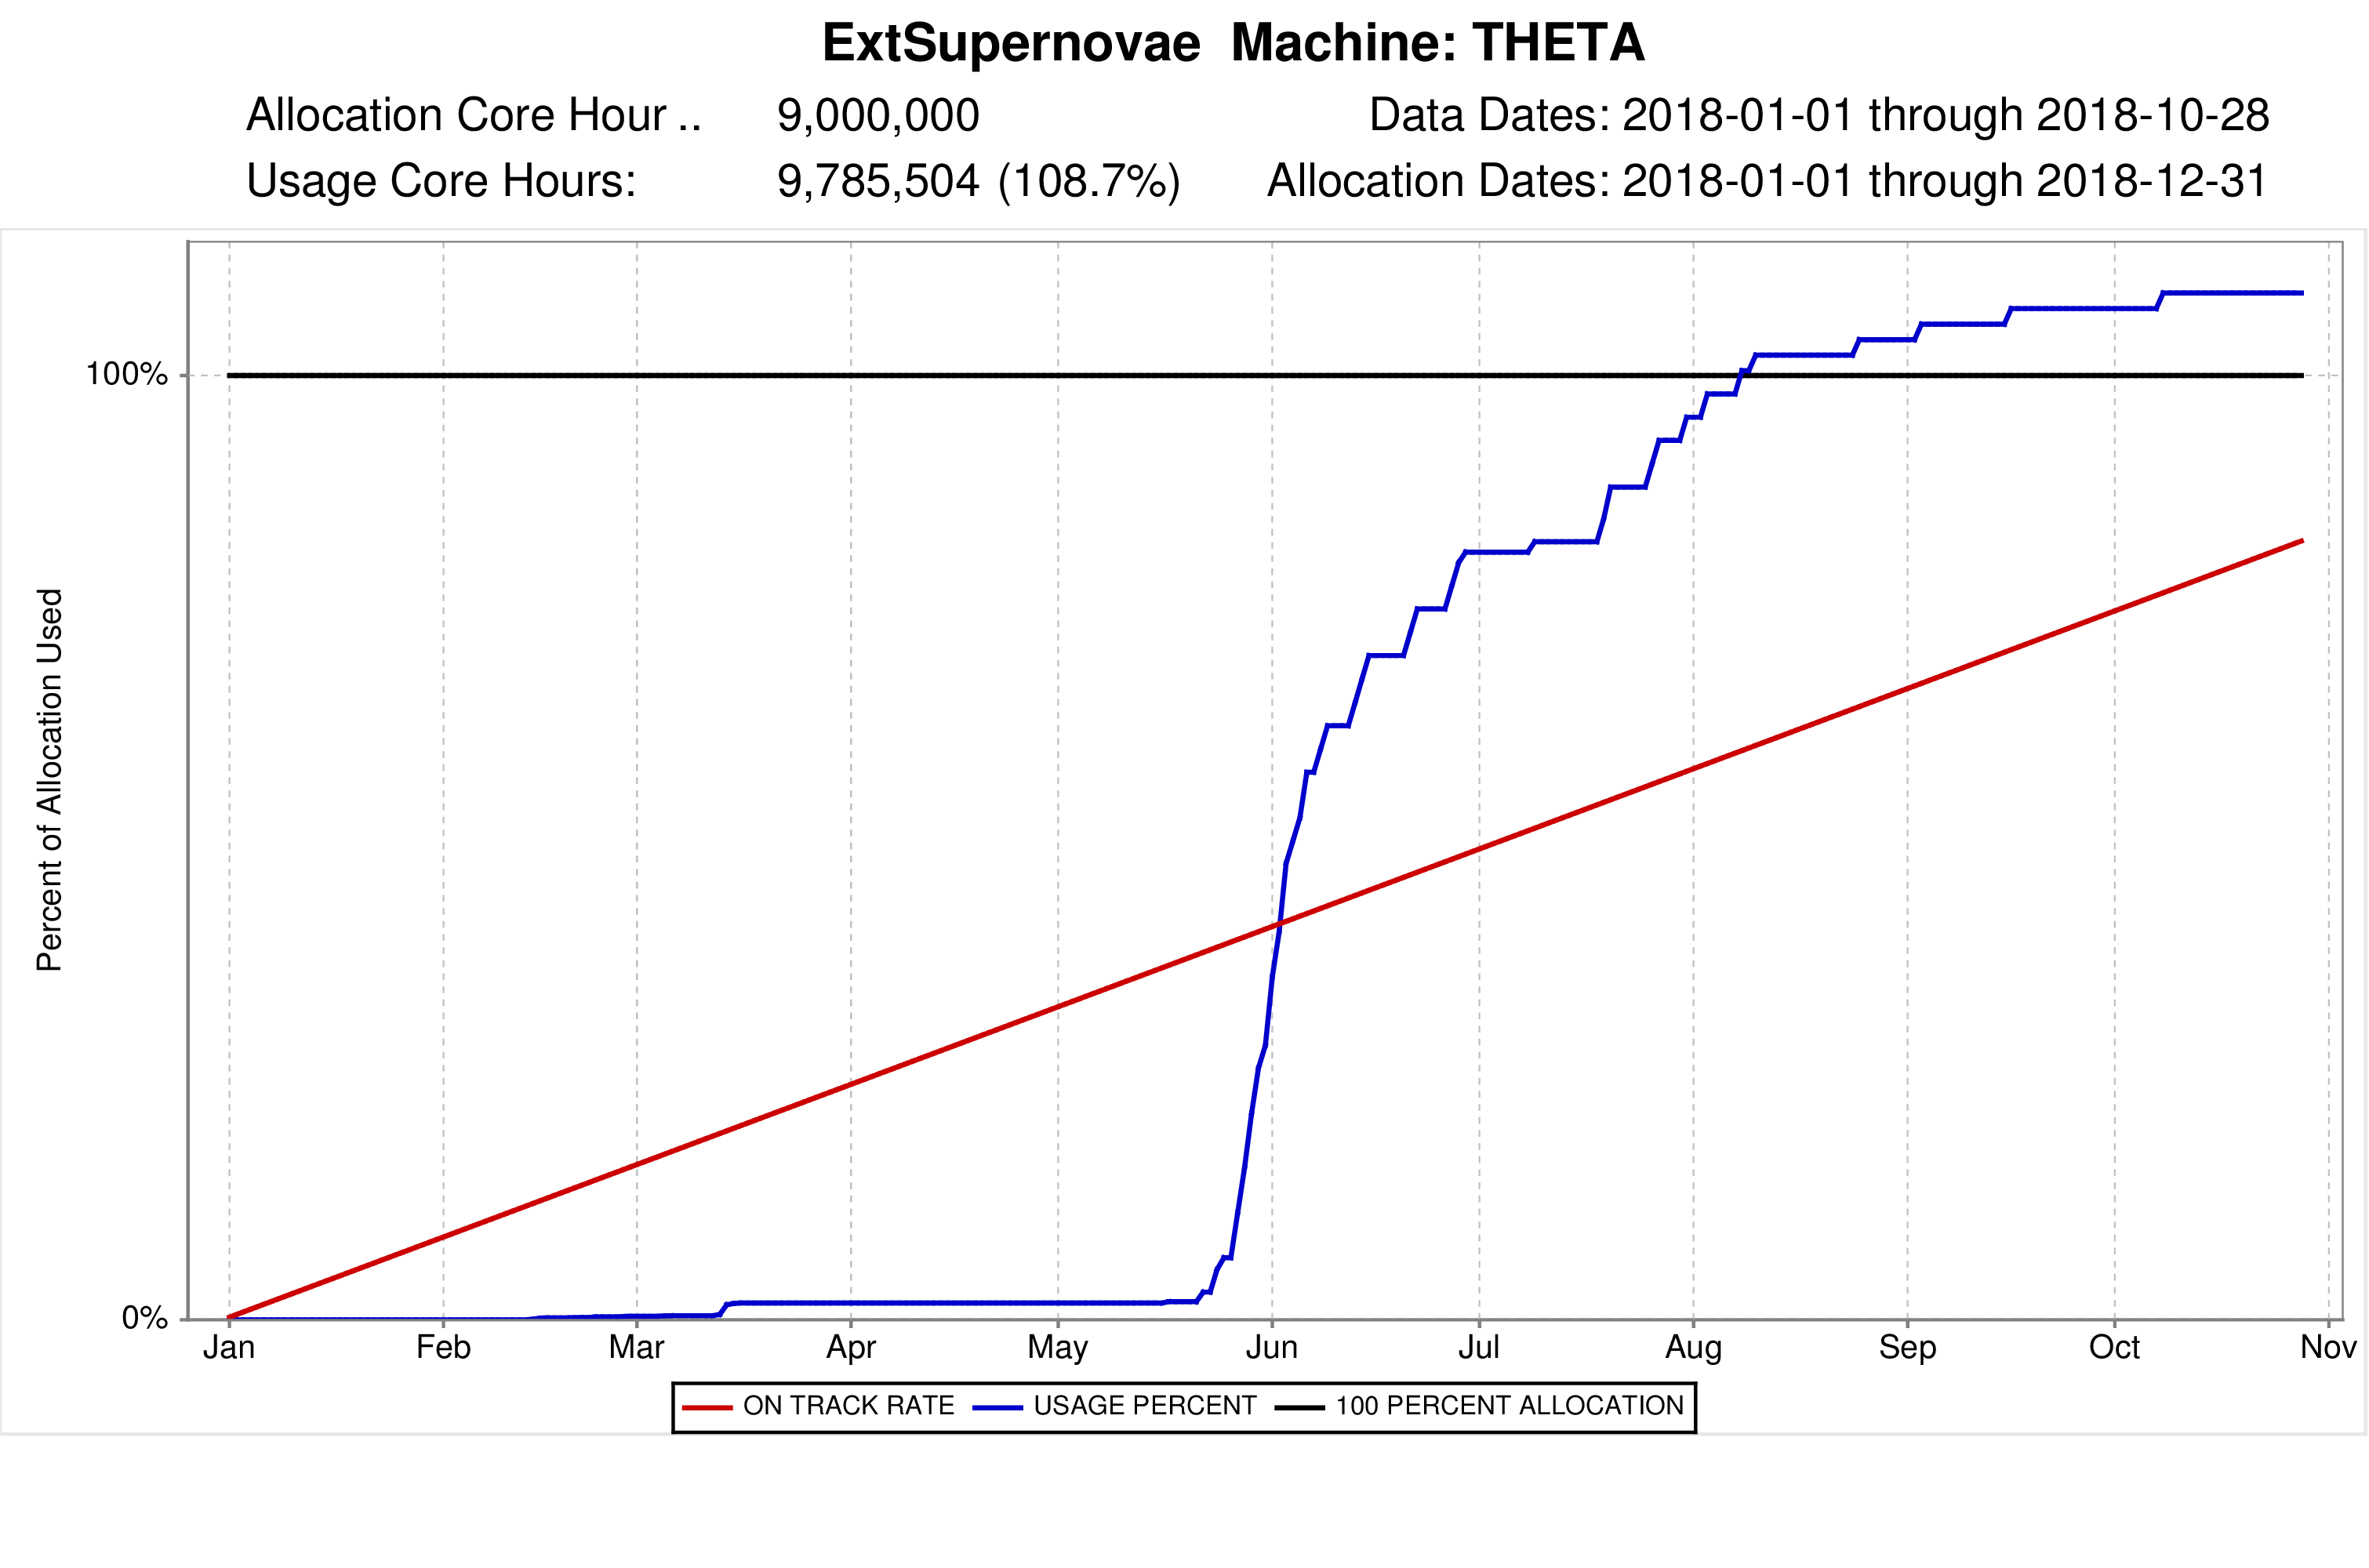
\includegraphics[width=3.25in]{on_track_graph}
    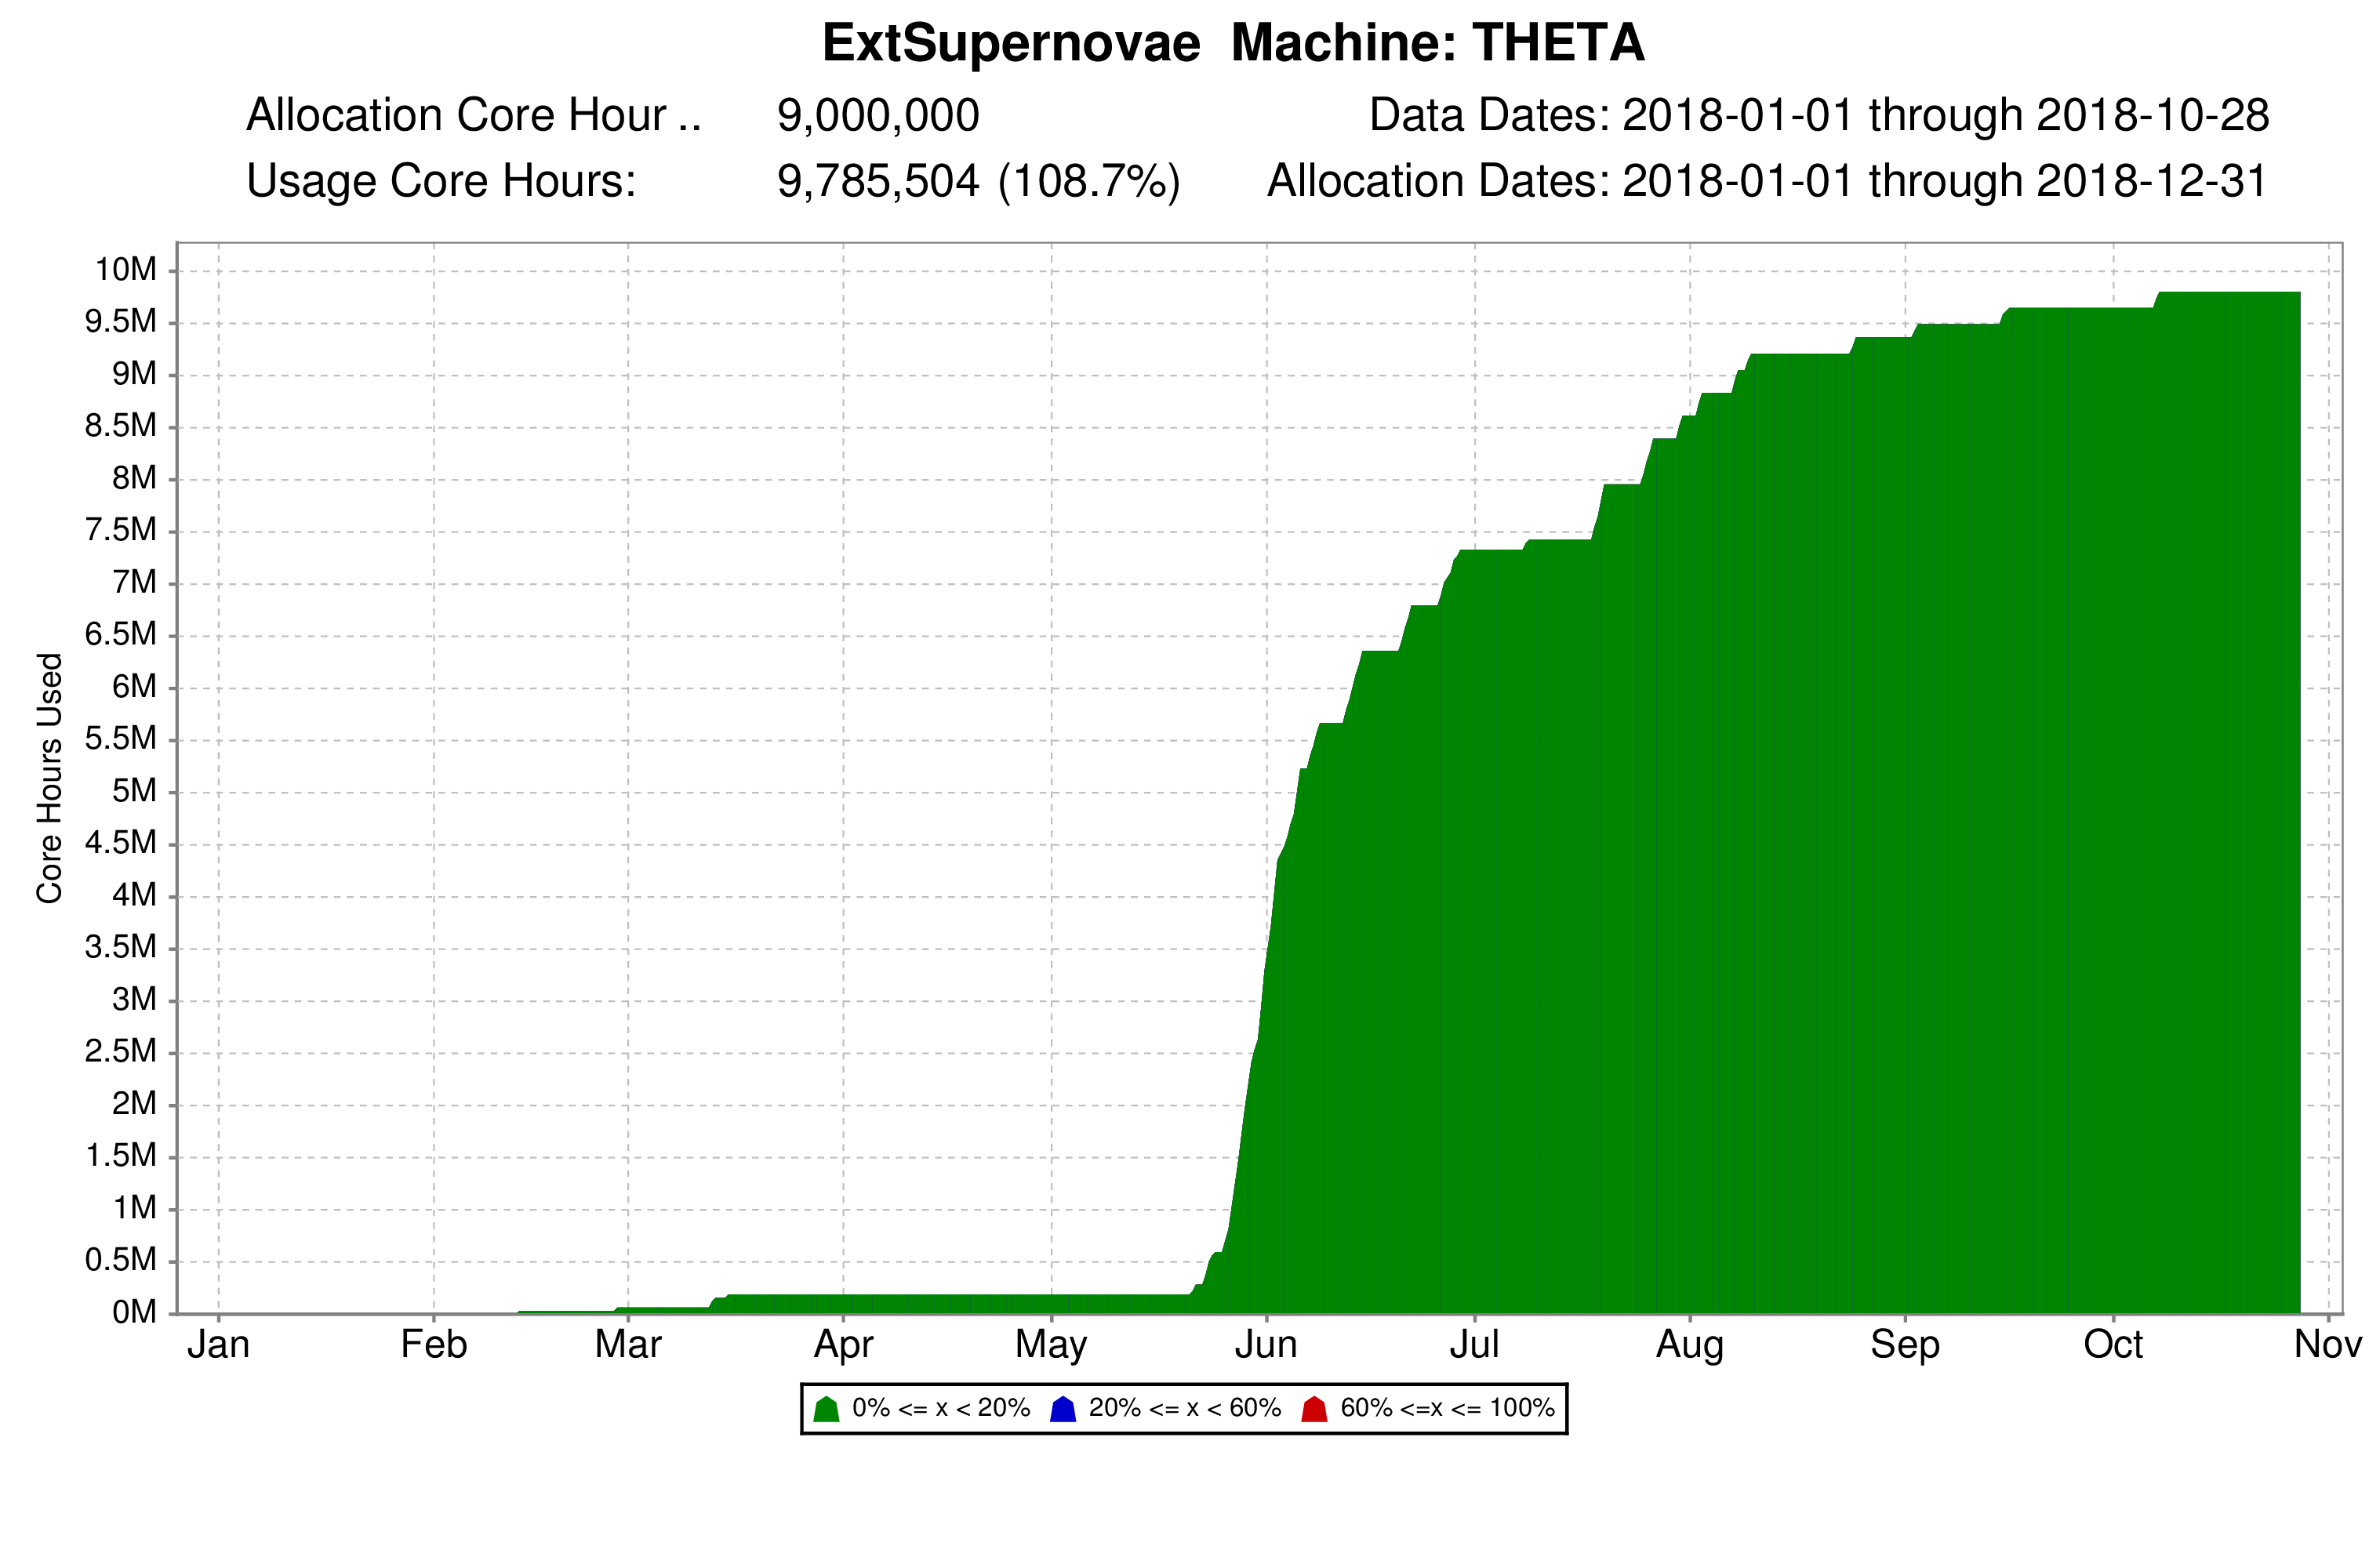
\includegraphics[width=3.25in]{categorized_hours_graph} 
  \end{tabular}
  \caption{Allocation usage.}
  \label{fig:usage}
\end{figure}

Thus far, we have expended 110.4M core-hours on Mira, 73.6\% of our 2018 allocation (see Figure \ref{fig:usage}).
We are slightly behind the ideal usage curve, but are catching up quickly.
Our 3D CCSN simulations have now grown to sufficient size that we are able to split them into two 8192-node runs, rather than one. 
We have also commenced a 3D massive star evolution simulation on 8192 nodes. 
This is rapidly accelerating our burn rate.
The vast majority of our usage on Mira has been at the capability level.


We have so far expended 9.8M core-hours on Theta, 109\% of our 2018 allocation. 
We largely achieved our planned goals for simulations on Theta and are continuing our run there to even later tims in the backfill queue. 

We continue to debug an infrequent I/O error experienced during checkpoint reading at simulation initialization. 

% \begin{figure}
%   \begin{tabular}{cc} 
%     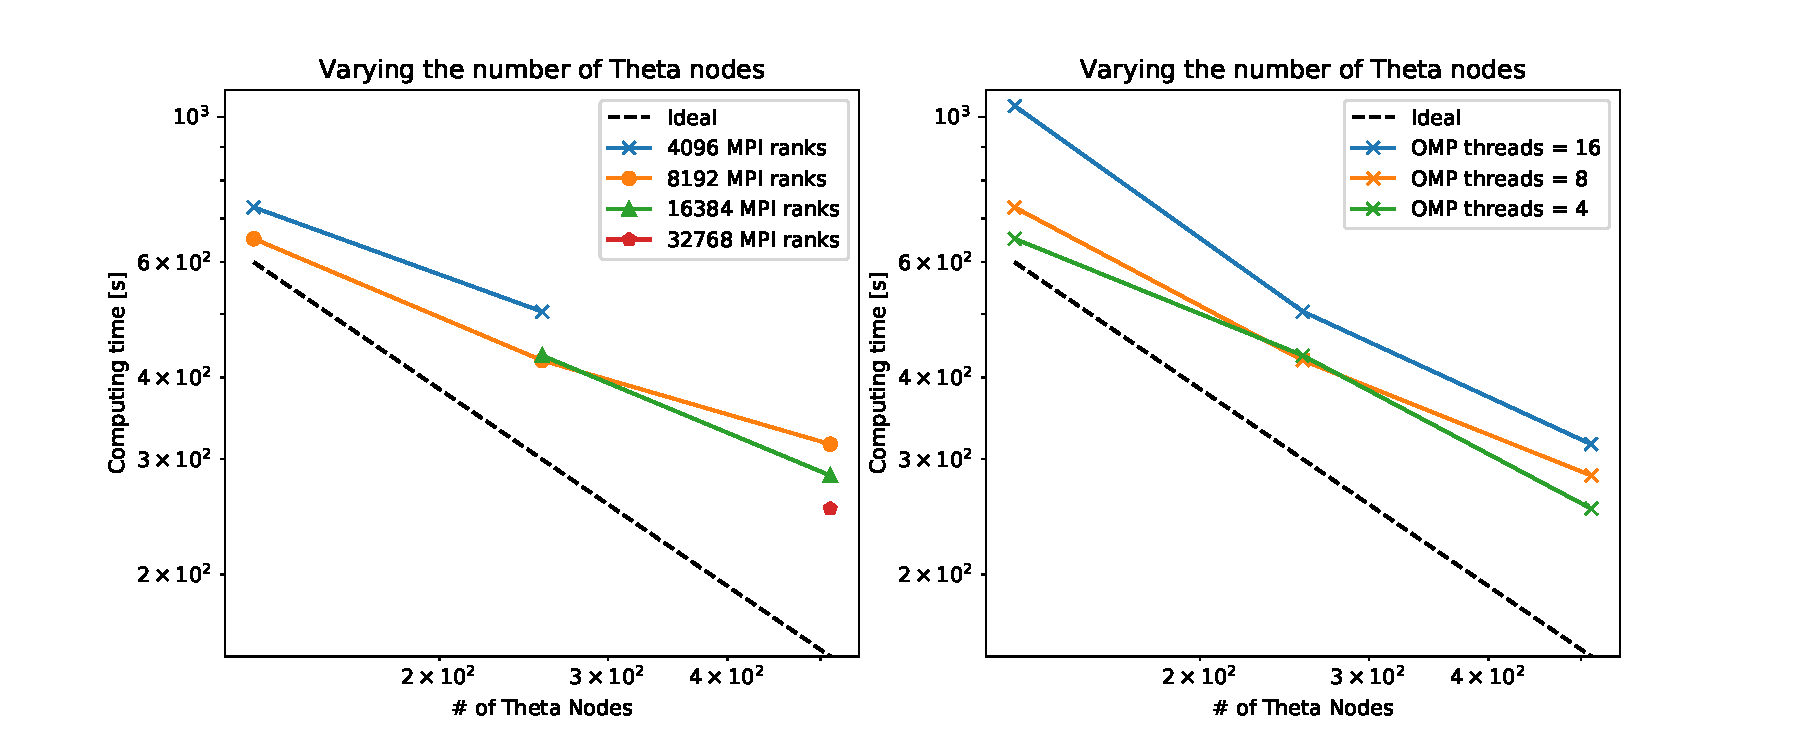
\includegraphics[width=6.5in]{./theta/fig_theta_scaling_j4.pdf}
%   \end{tabular}
%   \caption{Weak scaling test on Theta. different colors represent different combinations of MPI and OpenMP tasks. }
%   \label{fig:theta}
% \end{figure}




%%%%%%%%%%%%%%%%%%%%%%%%%%%%%%%%%
\section{Report on Project Milestones}
%%%%%%%%%%%%%%%%%%%

Our milestones for Year 1, and corresponding progress, are:
\begin{enumerate}
  \item {\it 3D simulations of magnetorotational core-collapse supernovae} -- These simulations are running at capability on Mira. The simulations have progressed sufficiently that we are beginning to see the impact of including rotation and magnetic fields. These simulations are on track to meet our scientific goals for 2018. The simulations on Theta involved rapidly-rotating initial conditions and have moved very quickly, thanks to our greater computational efficiency on Theta and higher queue throughput.
  \item {\it 3D simulations of iron core collapse in massive stars} -- We have commenced production runs in Q3. These simulations require far fewer restarts than the CCSN simulations and we anticipate completing one full-3D simulation by year's end.
  \item {\it High-resolution simulations of magnetorotational turbulence} -- This simulation has been started in Q3 and is growing in scale rapidly.
  \item {\it Develop SIMpliPy workflow tool} -- Work on this continues. 
  \item {\it Implement marching cubes for EOS and opacities} -- We have implemented other optimizations to the EOS and opacity table routines (primarily array re-ordering in the kernels) that has dramatically sped up this part of our simulations. So much so, it is not a significant fraction of runtime. Further optimization is on hold now.
\end{enumerate}



%%%%%%%%%%%%%%%%%%%%%%%%%%%%%%%%%
\section{Project Productivity}
%%%%%%%%%%%%%%%%%%%

\subsection{Primary}

\noindent {\bf Publications}
\begin{itemize}
  \item \href{https://ui.adsabs.harvard.edu/#abs/2018MNRAS.481.3293R/abstract}{``The antesonic condition for the explosion of core-collapse supernovae - I. Spherically symmetric polytropic models: stability and wind emergence''}, Raives, M. J., Couch, S. M., Greco, J. P., Pejcha, O., Thompson, T. A. 2018, {\itshape Monthly Notices of the Royal Astronomical Society}, 481, 3293 (2 citations)

\item \href{https://ui.adsabs.harvard.edu/#abs/2018ApJ...865...81O/abstract}{``Exploring Fundamentally Three-dimensional Phenomena in High-fidelity Simulations of Core-collapse Supernovae''}, O’Connor, E. P., Couch, S. M. 2018, {\itshape The Astrophysical Journal}, 865, 81 (3 citations)

\item \href{https://ui.adsabs.harvard.edu/#abs/2018JPhG...45j4001O/abstract}{``Global comparison of core-collapse supernova simulations in spherical symmetry''}, O’Connor, E., Bollig, R., Burrows, A., et al.\ 2018, {\itshape Journal of Physics G Nuclear Physics}, 45, 104001 (4 citations)

\item \href{https://ui.adsabs.harvard.edu/#abs/2018arXiv180610030P/abstract}{``The Impact of Different Neutrino Transport Methods on Multidimensional Core-collapse Supernova Simulations''}, Pan, K., Mattes, C., O'Connor, E. P., Couch, S. M., Perego, A., Arcones, A. 2018, {\itshape ArXiv e-prints}, arXiv:1806.10030 (2 citations)
  \item \href{http://adsabs.harvard.edu/abs/2018JPhG...45e3003R}{``Turbulence in Core-Collapse Supernovae''}, Radice, D., Abdikamalov, E., Ott, C. D., Moesta, P., Couch, S. M., Roberts, L. F. 2018, {\itshape Journal of Physics G}, 45, 053003 (3 citations)
  \item \href{https://ui.adsabs.harvard.edu/#abs/2018ApJ...857...13P/abstract}{``Equation of State Dependent Dynamics and Multi-messenger Signals from Stellar-mass Black Hole Formation''}, Pan, K., Liebend\"orfer, M., Couch, S. M., Thielemann, F. 2018, {\itshape The Astrophysical Journal}, 857, 13 (4 citations)
\end{itemize}

\noindent {\bf Presentations}

\begin{itemize}
  \item ``Understanding Massive Stellar Death: Predictive Simulation of Core-collapse Supernovae,'' S.M. Couch, Oskar Klein Centre Colloquium, Stockholm University, Stockholm, Sweden, October 2018
  \item ``Understanding Massive Stellar Death: Predictive Simulation of Core-collapse Supernovae,'' S.M. Couch, Physics Colloquium, Notre Dame University, Notre Dame, IN, October 2018
  % \item ``Understanding Massive Stellar Death: Predictive Simulation of Core-collapse Supernovae,'' S.M. Couch, CCAPP Seminar, Ohio State University, Columbus, OH, April 2018
  % \item ``Understanding Massive Stellar Death: Predictive Simulation of Core-collapse Supernovae,'' S.M. Couch, Physics and Astronomy Colloquium, Louisiana State University, Baton Rouge, LA, March 2018
  % \item ``Understanding Massive Stellar Death: Predictive Simulation of Core-collapse Supernovae,'' S.M. Couch, Physics and Astronomy Colloquium, University of Alabama, Tuscaloosa, AL, February 2018
\end{itemize}

\subsubsection{Secondary}

\begin{itemize}
  \item Co-I and postdoc Kuo-Chuan Pan will start a faculty position at National Tsing Hua University in Taiwan this summer.
  \item Co-I and postdoc MacKenzie Warren has won a prestigious NSF Postdoctoral Fellowship.
\end{itemize}

\section{Center Feedback}

Our catalyst, Adrian Pope, has been extremely helpful.
We have been experience occasional, seemingly random, I/O errors when reading large checkpoint files at startup.
He is helping us debug this, but the error is difficult to reproduce reliably.
This has slightly slowed progress, but not ground it to a halt.


\section{Code Description and Characterization}

\texttt{FLASH} is a highly capable, fully modular, extensible,
community code that is widely used in astrophysics, cosmology, fluid
dynamics, and plasma physics, and other fields.  The capabilities of
the FLASH code include adaptive mesh refinement (AMR), several
self-gravity solvers, an advection-diffusion-reaction (ADR) flame
model, an accurate and detailed treatment of nuclear burning, and a
sophisticated two-moment neutrino transport scheme based on an
explicit hyperbolic solver.  The neutrino interactions are included
through the open-source neutrino interaction library
\texttt{NuLib}. During Year 2 of this allocation we enhanced the
performance of the two-moment neutrino transport scheme significantly
as well as upgraded the transport to now include full velocity and
gravitational red-shift dependence in the evolution equations.

\texttt{FLASH} is written in modern Fortran, with some utility
functions written in C, and a build system written in Python.  It
requires MPI library support, and either HDF5 or P-NetCDF for I/O.
Additional mathematical software, such as \texttt{Hypre}, may be
required to configure \texttt{FLASH} for particular simulations.

Algorithm classes used within \texttt{FLASH} include Sparse Linear
Algebra solvers, FFT, active and passive particles, structured grids,
and AMR.



\end{document}
